%\documentclass[a3,portrait]{a0poster}
%\documentclass[a3,landscape]{a0poster}
\documentclass[a3,portrait]{a0poster}
\nonstopmode
%\documentclass[portrait]{a0poster}
%\documentclass[a0poster]{article}

\usepackage[T1]{fontenc}
%\usepackage[koi8-r]{inputenc}
\usepackage[latin1]{inputenc}
%\usepackage[utf8]{inputenc}
%\usepackage[russian]{babel}
%\usepackage[french]{babel}
\usepackage[english]{babel}
%\usepackage[T1]{fontenc}

\usepackage[usenames,dvipsnames]{color}

\usepackage{pbsi}
%\usepackage{mathptmx}
%\usepackage{tgothic}
%\usepackage{vicent}
\usepackage{chancery}
\usepackage{fourier}


\usepackage{eso-pic}
\usepackage[pdftex]{graphicx}
%\usepackage{color}
%\usepackage[dvipsnames]{color}



\definecolor{MyDarkBlue}{rgb}{0,0.08,0.45}
\definecolor{IITPLightBlue}{rgb}{0.27,0.45,0.73}
\definecolor{IITPBlue}{rgb}{0.25,0.41,0.68}
\definecolor{IITPDarkBlue}{rgb}{0.19,0.32,0.50}
\definecolor{IITPDarkDarkBlue}{rgb}{0.15,0.24,0.37}
%\definecolor{MyDarkGreen}{rgb}{0,0.3,0}
\definecolor{MyDarkGreen}{rgb}{0.3,0.5,0.2}
\definecolor{ElectronGreenLight}{rgb}{0,0.6,0.0}
\definecolor{ElectronGreen}{rgb}{0,0.42,0.0}
\definecolor{ElectronGreenDark}{rgb}{0,0.35,0.0}
\definecolor{PomegranateRed}{rgb}{0.7,0.1,0.1}

\input dvipsnam.def
%\usepackage[OT1]{fontenc}
\usepackage[T1]{fontenc}


%\usepackage{nimbus}
%\renewcommand*\familydefault{\sfdefault} %% Only if the base font of the document is to be sans serif
%\usepackage[T1]{fontenc}

\newcommand\notyet[1]{ }

%\oddsidemargin -1.5cm

%\textwidth 38cm
%\textheight 28cm


\textwidth 24cm
\textheight 38cm

%\textwidth 42cm
%\textheight 29.7cm

%\oddsidemargin 15mm
%\evensidemargin 15mm
\topmargin 4cm

\setlength{\parindent}{0mm}
\setlength{\parskip}{2pt}

%\setlength{\baselineskip}{10pt}

\pagestyle{empty}

\providecommand{\LenToUnit}[1]{#1\@gobble}
\newcommand{\PRH}[5]{%
\AddToShipoutPicture*{\put(\LenToUnit{#3},\LenToUnit{#4}){%
     \parbox[b][\paperheight]{\paperwidth}{%       
       \vfill
       \centering
       \includegraphics[width=#1,height=#2,%
                        keepaspectratio]{#5}%
       \vfill
     }}}
}  

\newcommand\BackgroundStrip{
\put(-8,420){
\parbox[b][\paperheight]{\paperwidth}{%
\vfill
\centering
\vfill
}}}

\newcommand\BackgroundPic{
\put(-4,0){
%\put(-8,-60){
\parbox[b][\paperheight]{\paperwidth}{%
\vfill
\centering
%%AC: takes a lot of time:
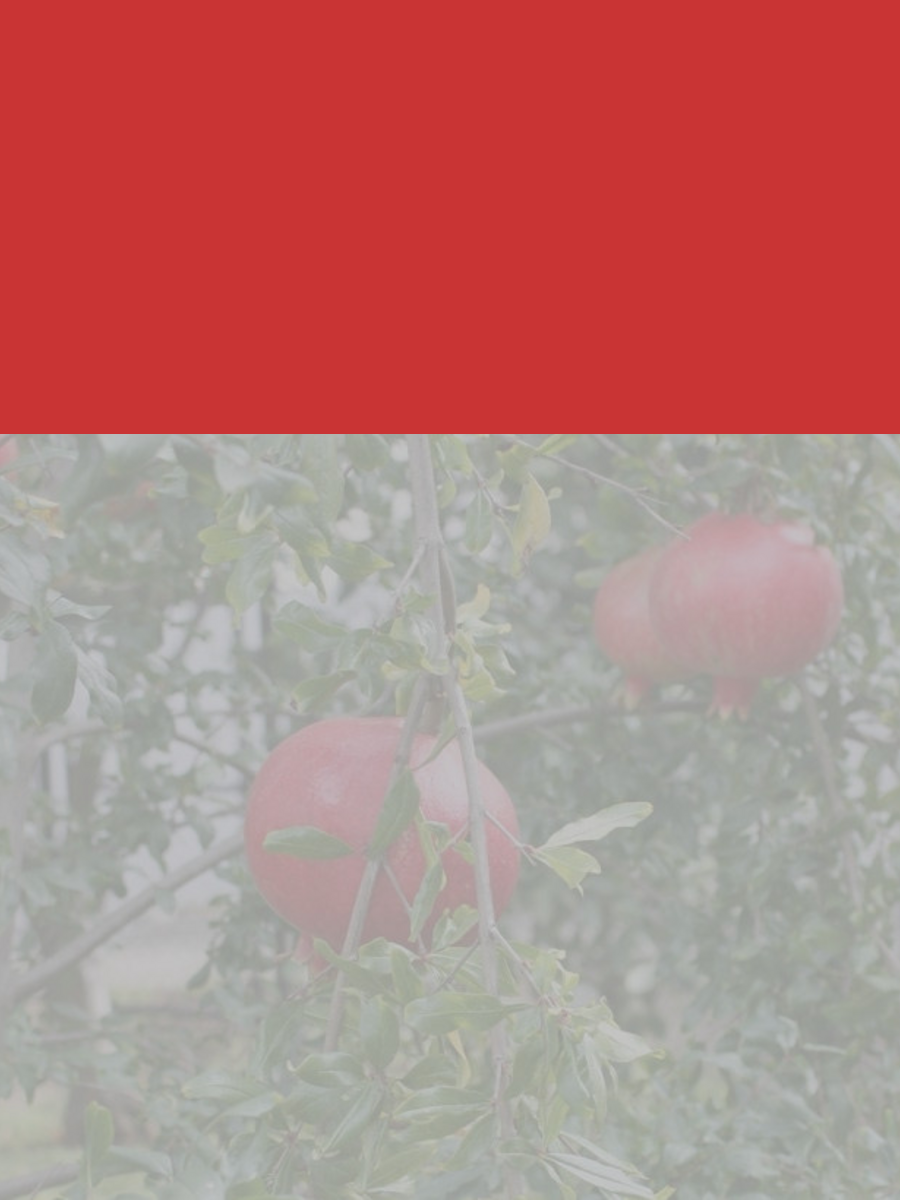
\includegraphics{p5.png}%
%\includegraphics{piter-neva-2018br.png}%
%\includegraphics{buslaev.png}%
\vfill
}}}


\begin{document}

\footnotesize

\AddToShipoutPicture{\BackgroundStrip}

\AddToShipoutPicture{\BackgroundPic}

\notyet{\bsifamily
\footnotesize
\color{GreenYellow}GreenYellow
\color{Yellow}Yellow
\color{Goldenrod}Goldenrod
\color{Dandelion}Dandelion
\color{Apricot}Apricot
\color{Peach}Peach
\color{Melon}Melon
\color{YellowOrange}YellowOrange
\color{Orange}Orange

\color{BurntOrange}BurntOrange
\color{Bittersweet}Bittersweet
\color{RedOrange}RedOrange
\color{Mahogany}Mahogany
\color{Maroon}Maroon
\color{BrickRed}BrickRed
\color{Red}Red
\color{OrangeRed}OrangeRed

\color{RubineRed}RubineRed
\color{WildStrawberry}WildStrawberry
\color{Salmon}Salmon
\color{CarnationPink}CarnationPink
\color{Magenta}Magenta
\color{VioletRed}VioletRed
\color{Rhodamine}Rhodamine

\color{Mulberry}Mulberry
\color{RedViolet}RedViolet
\color{Fuchsia}Fuchsia
\color{Lavender}Lavender
\color{Thistle}Thistle
\color{Orchid}Orchid
\color{DarkOrchid}DarkOrchid
\color{Purple}Purple
\color{Plum}Plum

\color{Violet}Violet
\color{RoyalPurple}RoyalPurple
\color{BlueViolet}BlueViolet
\color{Periwinkle}Periwinkle
\color{CadetBlue}CadetBlue
\color{CornflowerBlue}CornflowerBlue
\color{MidnightBlue}MidnightBlue

\color{NavyBlue}NavyBlue
\color{RoyalBlue}RoyalBlue
\color{Blue}Blue
\color{Cerulean}Cerulean
\color{Cyan}Cyan
\color{ProcessBlue}ProcessBlue
\color{SkyBlue}SkyBlue
\color{Turquoise}Turquoise
\color{TealBlue}TealBlue

\color{Aquamarine}Aquamarine
\color{BlueGreen}BlueGreen
\color{Emerald}Emerald
\color{JungleGreen}JungleGreen
\color{SeaGreen}SeaGreen
\color{Green}Green
\color{ForestGreen}ForestGreen
\color{PineGreen}PineGreen

\color{LimeGreen}LimeGreen
\color{YellowGreen}YellowGreen
\color{SpringGreen}SpringGreen
\color{OliveGreen}OliveGreen
\color{RawSienna}RawSienna
\color{Sepia}Sepia
\color{Brown}Brown
\color{Tan}Tan
\color{Gray}Gray

\vskip -7.25cm
%\end{document}

}%\notyet



\begin{center}

%\vskip -50mm

\ \vskip -15mm


%\color{MyDarkGreen}
%\color{Sepia}
%\color{ForestGreen}
%\color{Mahogany}
%\color{IITPBlue}


%\color{OrangeRed}
\color{white}
%\color{IITPLightBlue}
{\bfseries\LARGE
Ninth Annual Texas Analysis and
}

\vskip 4mm

{\bfseries\LARGE Mathematical Physics Symposium
}

%\vskip 6mm

%\color{OrangeRed}
%{%\titlefont
%\scshape\bf\large
%\qquad
%Buslaev
%}

\vskip 1cm

%\color{OrangeRed}
%\color{IITPDarkDarkBlue}


\mbox{
\textbf{
\Large
\quad
Texas A\&M University
}
}

\vskip 1cm

\mbox{
\textbf{
\large
%\normalsize
\quad
9\,--11 \ February \ 2024
}
}


\end{center}



\medskip

%\scriptsize
%\footnotesize
%\titlefontsmall
%\color{MyDarkBlue}
%\color{RoyalBlue}
%\color{Blue}
%\color{WildStrawberry}
\color{PomegranateRed}
%\color{RubineRed}
%\color{NavyBlue}


%\PRH{300pt}{570pt}{-85mm}{15mm}{mi-749}

%\PRH{600pt}{638pt}{-120mm}{-35mm}{buslaev.png}

%\PRH{400pt}{600pt}{120mm}{-35mm}{psi.png}

\vskip 5cm

%%\hskip 26cm{\bsifamily\normalsize Invited speakers}
\hskip 7cm{\bsifamily\large Invited Speakers}

\vskip 1cm

%\bfseries\tiny
\bf
%\tiny
%\footnotesize
%\scriptsize
\normalsize
\Large
\hskip -1.9cm
%\hskip 15cm
\begin{tabular}{r}
Nabile BOUSSAID
%Universit\'{e} Franche-Comte -- Besan\c{c}on
\\
Chris JUDGE
%Indiana University
\\
Eugenia MALINNIKOVA
%Stanford University
\\
Andrea NAHMOD
%University of Massachussetts -- Amherst
\\
Iosif POLTEROVICH
%Universit\'{e} de Montr\'{e}al
\\
Jacob SHAPIRO
%Princeton University
\\
Andras VASY
%Stanford University
\end{tabular}
%\hskip 1mm
\begin{tabular}{l}
\it
Universit\'{e} Franche-Comte
% (Besan\c{c}on)
\\
\it
Indiana University
\\
\it
Stanford University
\\
\it
University of Massachussetts
%(Amherst)
\\
\it
Universit\'{e} de Montr\'{e}al
\\
\it
Princeton University
\\
\it
Stanford University
\end{tabular}


\vskip 3cm

\color{MidnightBlue}

%\footnotesize
%\scriptsize
\normalsize
%\small

%\hskip 4cm
%\begin{tabular}{r}
{\bsifamily Organizers:}
Dean Baskin, Gregory Berkolaiko, Andrew Comech,

Peter Kuchment,
Wencai Liu, Jonas L\"{u}hrmann, Minh-Binh Tran
%\end{tabular}


\vskip 0.5cm

\hskip 6cm
Supported by %% NSF and
Texas A\&M University


\vskip 1cm

\hskip 11cm
\mbox{
\normalsize
comech.sdf.org/texamp-2024
}

\vskip -16mm
\hskip 22.5cm
\mbox{

\includegraphics[height=15mm]{texamp-2024-qr.png}
}

\end{document}
